%
\documentclass[11pt,stdletter,orderfromtodate,sigleft,twoside]{report}

\usepackage[letterpaper,margin=0.8in,top=0.9in]{geometry}  % --- 
%\geometry{textwidth=17cm,margin=2cm}                      % --- 
\usepackage[spanish]{babel}                                % Language accents 
\usepackage[pdftex]{graphicx}                              % --- 
\usepackage{setspace}                                      % --- 
\usepackage[T1]{fontenc}                                   % --- 
\usepackage[utf8]{inputenc}                                % --- 
\usepackage{blindtext, xfrac}                              % --- 
\usepackage{parskip}                                       % --- 
\usepackage{lastpage}                                      % --- 
\usepackage{multirow,array,tabularx}                       % --- 
\usepackage{enumitem}                                      % --- 
\usepackage{framed}                                        % ---
\usepackage{lipsum}                                        % ---
\usepackage{listings}                                      % ---


% Fuentes
% opcion 1
%\usepackage{lmodern}
% opcion 2
\usepackage[sfdefault,scaled=.85]{FiraSans}
\usepackage{newtxsf}

%\usepackage{etoolbox}
%\patchcmd{\thebibliography}{\chapter*}{\section*}{}{}
\usepackage[
    style=authoryear,%numeric,
    %bibstyle=numeric,
    citestyle=apa,
    sortcites = true,
    sorting=nyt,
    natbib = false,
    backend=biber,
    isbn=false,
    url=false,
    doi=true,
    eprint=false,
    bibencoding=utf8
]{biblatex}
\addbibresource{referencias.bib}
\defbibheading{secbib}[\bibname]{%
  \section*{#1}%
  \markboth{#1}{#1}}


\usepackage[pdfpagelabels,final,bookmarks=true,plainpages=false]{hyperref}
\usepackage[dvipsnames,svgnames,x11names,hyperref]{xcolor}
\hypersetup{colorlinks=true,citecolor=BlueViolet,linkcolor=Blue,urlcolor=PineGreen,filecolor=Green}
% -------------------------------------------------------------------------
\usepackage[spanish]{cleveref}  % debe ser cargado despues de hyperref
\input{crefnames.tex}
% -------------------------------------------------------------------------

\definecolor{codegreen}{rgb}{0,0.6,0}
\definecolor{codegray}{rgb}{0.5,0.5,0.5}
\definecolor{codepurple}{rgb}{0.58,0,0.82}
\definecolor{backcolour}{rgb}{0.95,0.95,0.92}

\lstdefinestyle{mystyle}{
    backgroundcolor=\color{backcolour},   
    commentstyle=\color{codegreen},
    keywordstyle=\color{magenta},
    numberstyle=\tiny\color{codegray},
    stringstyle=\color{codepurple},
    basicstyle=\ttfamily\footnotesize,
    breakatwhitespace=false,         
    breaklines=true,                 
    captionpos=b,                    
    keepspaces=true,                 
    numbers=left,                    
    numbersep=5pt,                  
    showspaces=false,                
    showstringspaces=false,
    showtabs=false,                  
    tabsize=2
}

\lstset{style=mystyle}

\DeclareGraphicsExtensions{.pdf,.png,.jpg}
% Title Page
%\title{}
%\author{}

\setcounter{secnumdepth}{3}

\newcommand{\uncol}{Universidad Nacional de Colombia}
\newcommand{\facingbog}{Facultad de Ingeniería - Sede Bogotá}
\newcommand{\dimmbog}{Departamento de Ingeniería Mecánica y Mecatrónica}
\newcommand{\module}{Modelación Matemática}
\newcommand{\reportType}{Informe Taller 01}
\newcommand{\reportSubject}{Modelación Basada en EDOs}

%\renewcommand{\thechapter}{\Alph{chapter}}
\renewcommand{\thesection}{\arabic{section}}
\renewcommand{\thesubsubsection}{\arabic{section}\arabic{subsection}\arabic{subsubsection}}
\renewcommand*\familydefault{\sfdefault} %% Only if the base font of the document is to be sans serif
\renewcommand{\familydefault}{\sfdefault}
\setlength{\parindent}{0pt} % Default is 15pt.
\setlength{\parskip}{1ex}   % Default is      

\usepackage{fancyhdr}
\pagestyle{fancy}

\fancypagestyle{firststyle}
{
  \fancyhf{}
  %\fancyfoot[L]{\footnotesize }
  %\fancyfoot[C]{\footnotesize Actualización:  Octubre/2024}
  \fancyfoot[R]{\footnotesize Página \thepage\ de \pageref{LastPage}}
}

\fancypagestyle{declarationstyle}
{
  \fancyhf{}
  %\fancyfoot[L]{\footnotesize }
  \fancyfoot[C]{\footnotesize \reportType - \module}
  %\fancyfoot[R]{\footnotesize Página \thepage\ de \pageref{LastPage}}
}

\fancyhead{} % clear all header fields
\fancyhead[RO]{\footnotesize \module - \reportType}
\fancyhead[LE]{\footnotesize \reportSubject}
%\fancyhead[RO,LE]{\bfseries }
\fancyfoot{} % clear all footer fields
\fancyfoot[L]{\footnotesize Semestre 02 / 2024}
\fancyfoot[C]{\footnotesize Actualización:  Octubre/2024}
\fancyfoot[R]{\footnotesize Página \thepage\ de \pageref{LastPage}}
%\fancyfoot[LO,CE]{From: K. Grant}
\renewcommand{\headrulewidth}{0.4pt}
\renewcommand{\footrulewidth}{0.4pt}

\newenvironment{leftbox}[1]
 {\itemize[
    nosep,
    leftmargin=2pt,
    rightmargin=\dimexpr\textwidth-#1\relax,
    itemindent=\parindent,
    listparindent=\parindent,
  ]\item[]\relax}
 {\enditemize}

\newenvironment{rightbox}[1]
 {\itemize[
    nosep,
    leftmargin=\dimexpr\textwidth-#1\relax,
    rightmargin=2pt,
    itemindent=\parindent,
    listparindent=\parindent,
  ]\item[]\relax}
 {\enditemize}

\definecolor{softBackGround}{RGB}{170,207,238}

\begin{document}

%\thispagestyle{firststyle}
%\maketitle

%\begin{abstract}
%\end{abstract}

%%------------------------------- cover page ----------------------------------
\pagenumbering{Alph}
\begin{titlepage}
\center

\vspace*{-12mm}
{\huge \textbf{\textsc{\uncol}}}\\
{\Large \textbf{\textsc{\facingbog}}}\\[20mm]

\vfill


\includegraphics[width=0.2\textwidth]{./templateFigures/escudo.png}\\[20mm]

\vfill

\begin{framed}
{\Huge \textbf{\reportSubject}}\\[4mm]
{\huge \textbf{\reportType}}\\[4mm]
{\huge \textbf{\module}}
\end{framed}
\vspace{12mm}

\vfill

{\Large \textbf{Coordinacion curso:}}\\[4mm]
{\large Principal: Ing. Carlos Alberto Duque-Daza\\[2mm]
        Práctica: Ing. Juan Sebastian Hincapie}\\[12mm]

{\Large \textbf{Estudiantes/Autores}}\\[4mm]
{\large Nombre de Autor1 $<$email1@unal.edu.co$>$ $<$ID-Autor1$>$}\\[2mm]
{\large Nombre de Autor2 $<$email2@unal.edu.co$>$ $<$ID-Autor2$>$}\\[2mm]
{\large Nombre de Autor3 $<$email3@unal.edu.co$>$ $<$ID-Autor3$>$}\\[2mm]
{\large Nombre de Autor4 $<$email4@unal.edu.co$>$ $<$ID-Autor4$>$}\\[12mm]


\vfill
\begin{rightbox}{2.5cm}
    
\includegraphics[width=0.95\linewidth]{./templateFigures/moduleOwnershipGNUM.png}
\end{rightbox}
\vfill

%\renewcommand{\today}{15 de dezembro de 2023}
\today

\end{titlepage}
\newpage

%%------------------------------- contribution acknowledgements page ----------------------------------

\thispagestyle{declarationstyle}
\vspace*{12mm}
\begin{framed}
    {\Large \textbf{\textsc{Declaración de aportes y contribuciones}}}\\[8mm]

Los autores del presente informe declaramos que TODOS hemos aportado de manera
significativa a la elaboración del presente informe, y que por tanto cualquiera
de nosotros está en capacidad de presentar sustentación de forma individual del
contenido del presente documento.

En cualquier caso, las contribuciones específicas de cada uno de los autores al
presente documento se detallan en la siguiente tabla, pero manifestamos que
esta distribución de responsabilidades se hizo solamente para fines de
producción final del informe, y aceptamos que la componente de calificación
asociada a una posible sustentación puede recaer en cualquiera de nosotros de
forma individual.

\end{framed}

\vfill

\begin{framed}
    {\large \textbf{Nombre de Autor1:} An\'alisis de Caso 1; Programaci\'on de c\'odigos computacionales Caso 1; Redacci\'on de texto Caso 1; Elaboraci\'on de curva de post-procesamiento Caso 1}\\[2mm]
\end{framed}
\begin{framed}
    {\large \textbf{Nombre de Autor2:} An\'alisis de Caso 2; Programaci\'on de c\'odigos computacionales Caso 2; Redacci\'on de texto Caso 2; Elaboraci\'on de curva de post-procesamiento Caso 2}\\[2mm]
\end{framed}
\begin{framed}
    {\large \textbf{Nombre de Autor3:} Elaboraci\'on y procesamiento de documento en \LaTeX ; Elaboraci\'on conclusiones Caso 1; Verificaci\'on bibliograf\'ia Caso 1}\\[2mm]
\end{framed}
\begin{framed}
    {\large \textbf{Nombre de Autor4:} Elaboraci\'on y procesamiento de documento en \LaTeX ; Elaboraci\'on conclusiones Caso 2; Verificaci\'on bibliograf\'ia Caso 2}\\[2mm]
\end{framed}

\newpage


%%------------------------------- main contents  --------------------------d--------
\pagenumbering{arabic}

\section{Caso 01: Sistema de tanques interconectados}
A continuaci\'on se muestra una potencial estructura de informe, enfocado en
casos de estudio. Por estructuraci\'on, es mejor presentar el an\'aisis y
desarrollo de cada caso de manera independiente, incluso si esto implica
repetir subsecciones (al menos conceptualmente, pues el texto deber\'a ser
diferente, obviamente).
\medskip 

El primer p\'arrafo puede ser usado para dar una breve descripci\'on del caso,
as\'i como una contextualizaci\'on, en forma de descripci\'on, de los
requerimientos y elementos conocidos del mismo. El segundo p\'arrafo
introductorio de cada caso puede ser usado para presentar una breve revisi\'on
del estado del conocimiento (revisi\'on de bibliograf\'ia especializada en el
tema del caso explorado.
\medskip

\lipsum[1]
\medskip

\subsection{An\'alisis Preliminar: Elementos del Modelo.}
En esta secci\'on se deber\'ia discutir el proceso de identificaci\'on y
clasificaci\'on de variables del modelo, los principios de conservaci\'on que
se consideren relevantes, y las relaciones constitutivas adecuadas
consideradas. Debe argumentarse de manera adecuada la clasificaci\'on de
variables adoptada, as\'i como el conjunto de elementos seleccionado para el
modelo.
\medskip

\lipsum[2]
\medskip

\subsection{Modelo Matem\'atico}
En esta secci\'on se deber\'an presentar las diferentes expresiones
matem\'aticas construidas, seleccionadas y/o adoptadas para el modelamiento del
caso en discusi\'on. Tambi\'en ser\'a conveniente realizar un proceso de
an\'alisis dimensional del modelo matem\'atico y presentar potenciales
relaciones adimensionales resultantes del proceso de an\'alisis dimensional.
\medskip

Deber\'an usarse referencias a tablas, figuras, ecuaciones, y cualquier otro
entorno que implique numeraci\'on. Este simple ejemplo muestra como hacer
referencias cruzadas a ecuaciones en el texto, como se muestra en \cref{eq:01}
y en \cref{eq:conservationU,eq:conservationV}.

\begin{equation}
    \frac{\partial u}{\partial t} = \alpha \nabla^2 u
    \label{eq:01}
\end{equation}

\begin{align}
\nabla \cdot \mathbf{u} &= 0 \label{eq:conservationU}\\
\rho \left( \frac{\partial \mathbf{u}}{\partial t} + \mathbf{u} \cdot \nabla \mathbf{u} \right) &= - \nabla p + \mu \nabla^2 \mathbf{u}\label{eq:conservationV}
\end{align}

\lipsum[3]

Las ecuaciones deben ser referenciadas en el documento antes de que aparezcan
las ecuaciones mismas, en la medida de lo posible, como en el presente ejemplo
\cref{eq:OtraMasA,eq:OtraMasB}
\begin{align}
\frac{\partial \mathbf{u}}{\partial t} + (\mathbf{u} \cdot \nabla) \mathbf{u} &= - \frac{1}{\rho} \nabla p + \nu \nabla^2 \mathbf{u} + \mathbf{f}, 
\quad \mathrm{for} \quad \mathbf{x} \in \Omega, \label{eq:OtraMasA} \\
\nabla \cdot \mathbf{u} &= 0, \quad \mathrm{for} \quad \mathbf{x} \in \Omega, \label{eq:OtraMasB} 
\end{align}

\subsection{Implementaci\'on Computacional}
En esta secci\'on pueden presentarse de manera suscinta los c\'odigos
implementados para el an\'alisis del caso. En cualquier caso, deber\'a  hacerse
una discusi\'on corta acerca de los m\'etodos num\'ericos usados para la
soluci\'on del caso, as\'i como  cualquier consideraci\'on digna de menci\'on
respecto a la estructura algoritmica usada en los c\'odigos presentados.

C\'odigos cortos pueden ser incluidos por completo en el documento con un
entorno tipo \emph{listing}, como se muestra a continuaci\'on en \cref{lst:code01}:
\lstinputlisting[language=Python, label=lst:code01, 
    caption= Ejemplo de inclusi\'on de c\'odigo corto]{./codes/forLoops.py}

Inclusi\'on de porciones espec\'ificas de c\'odigos m\'as extensos se puede
hacer como se indica a continuaci\'on (ver \cref{lst:code02}):

\begin{verbatim}
\lstinputlisting[language=Python,firstline=4,lastline=25,label=lst:code02,
        caption= Ejemplo de inclusi\'on de ... ]{./codes/getGradingFactor.py}
\end{verbatim}

\lstinputlisting[
                language=Python, 
                firstline=4,
                lastline=25,
                label=lst:code02,
                caption= Ejemplo de inclusi\'on de porci\'on de c\'odigo largo]
                {./codes/getGradingFactor.py}
\subsection{Resultados}
Se sugiere tener una secci\'on dedicada exclusivamente a la presentaci\'on de
los resultados obtenidos, as\'i como a la discusi\'on de tendencias
observadas(a partir de los resultados), o a la observaci\'on de comportamientos
que puedan ser considerados an\'omalos o contrarios a las observaciones
documentadas por la bibliograf\'ia.  Igualmente, es indispensable que todas las
gráficas y curvas incluidas en el informe tengan una resolución adecuada, y las
etiquetas e indicadores de escalas, as\'i como t\'itulos de gr\'aficos, tengan
un tama\~no adecuado para una f\'acil lectura, como se muestra en el ejemplo de
la \cref{fig:figuraEjemplo00}

\begin{figure}[!hbt]
    \begin{center}
        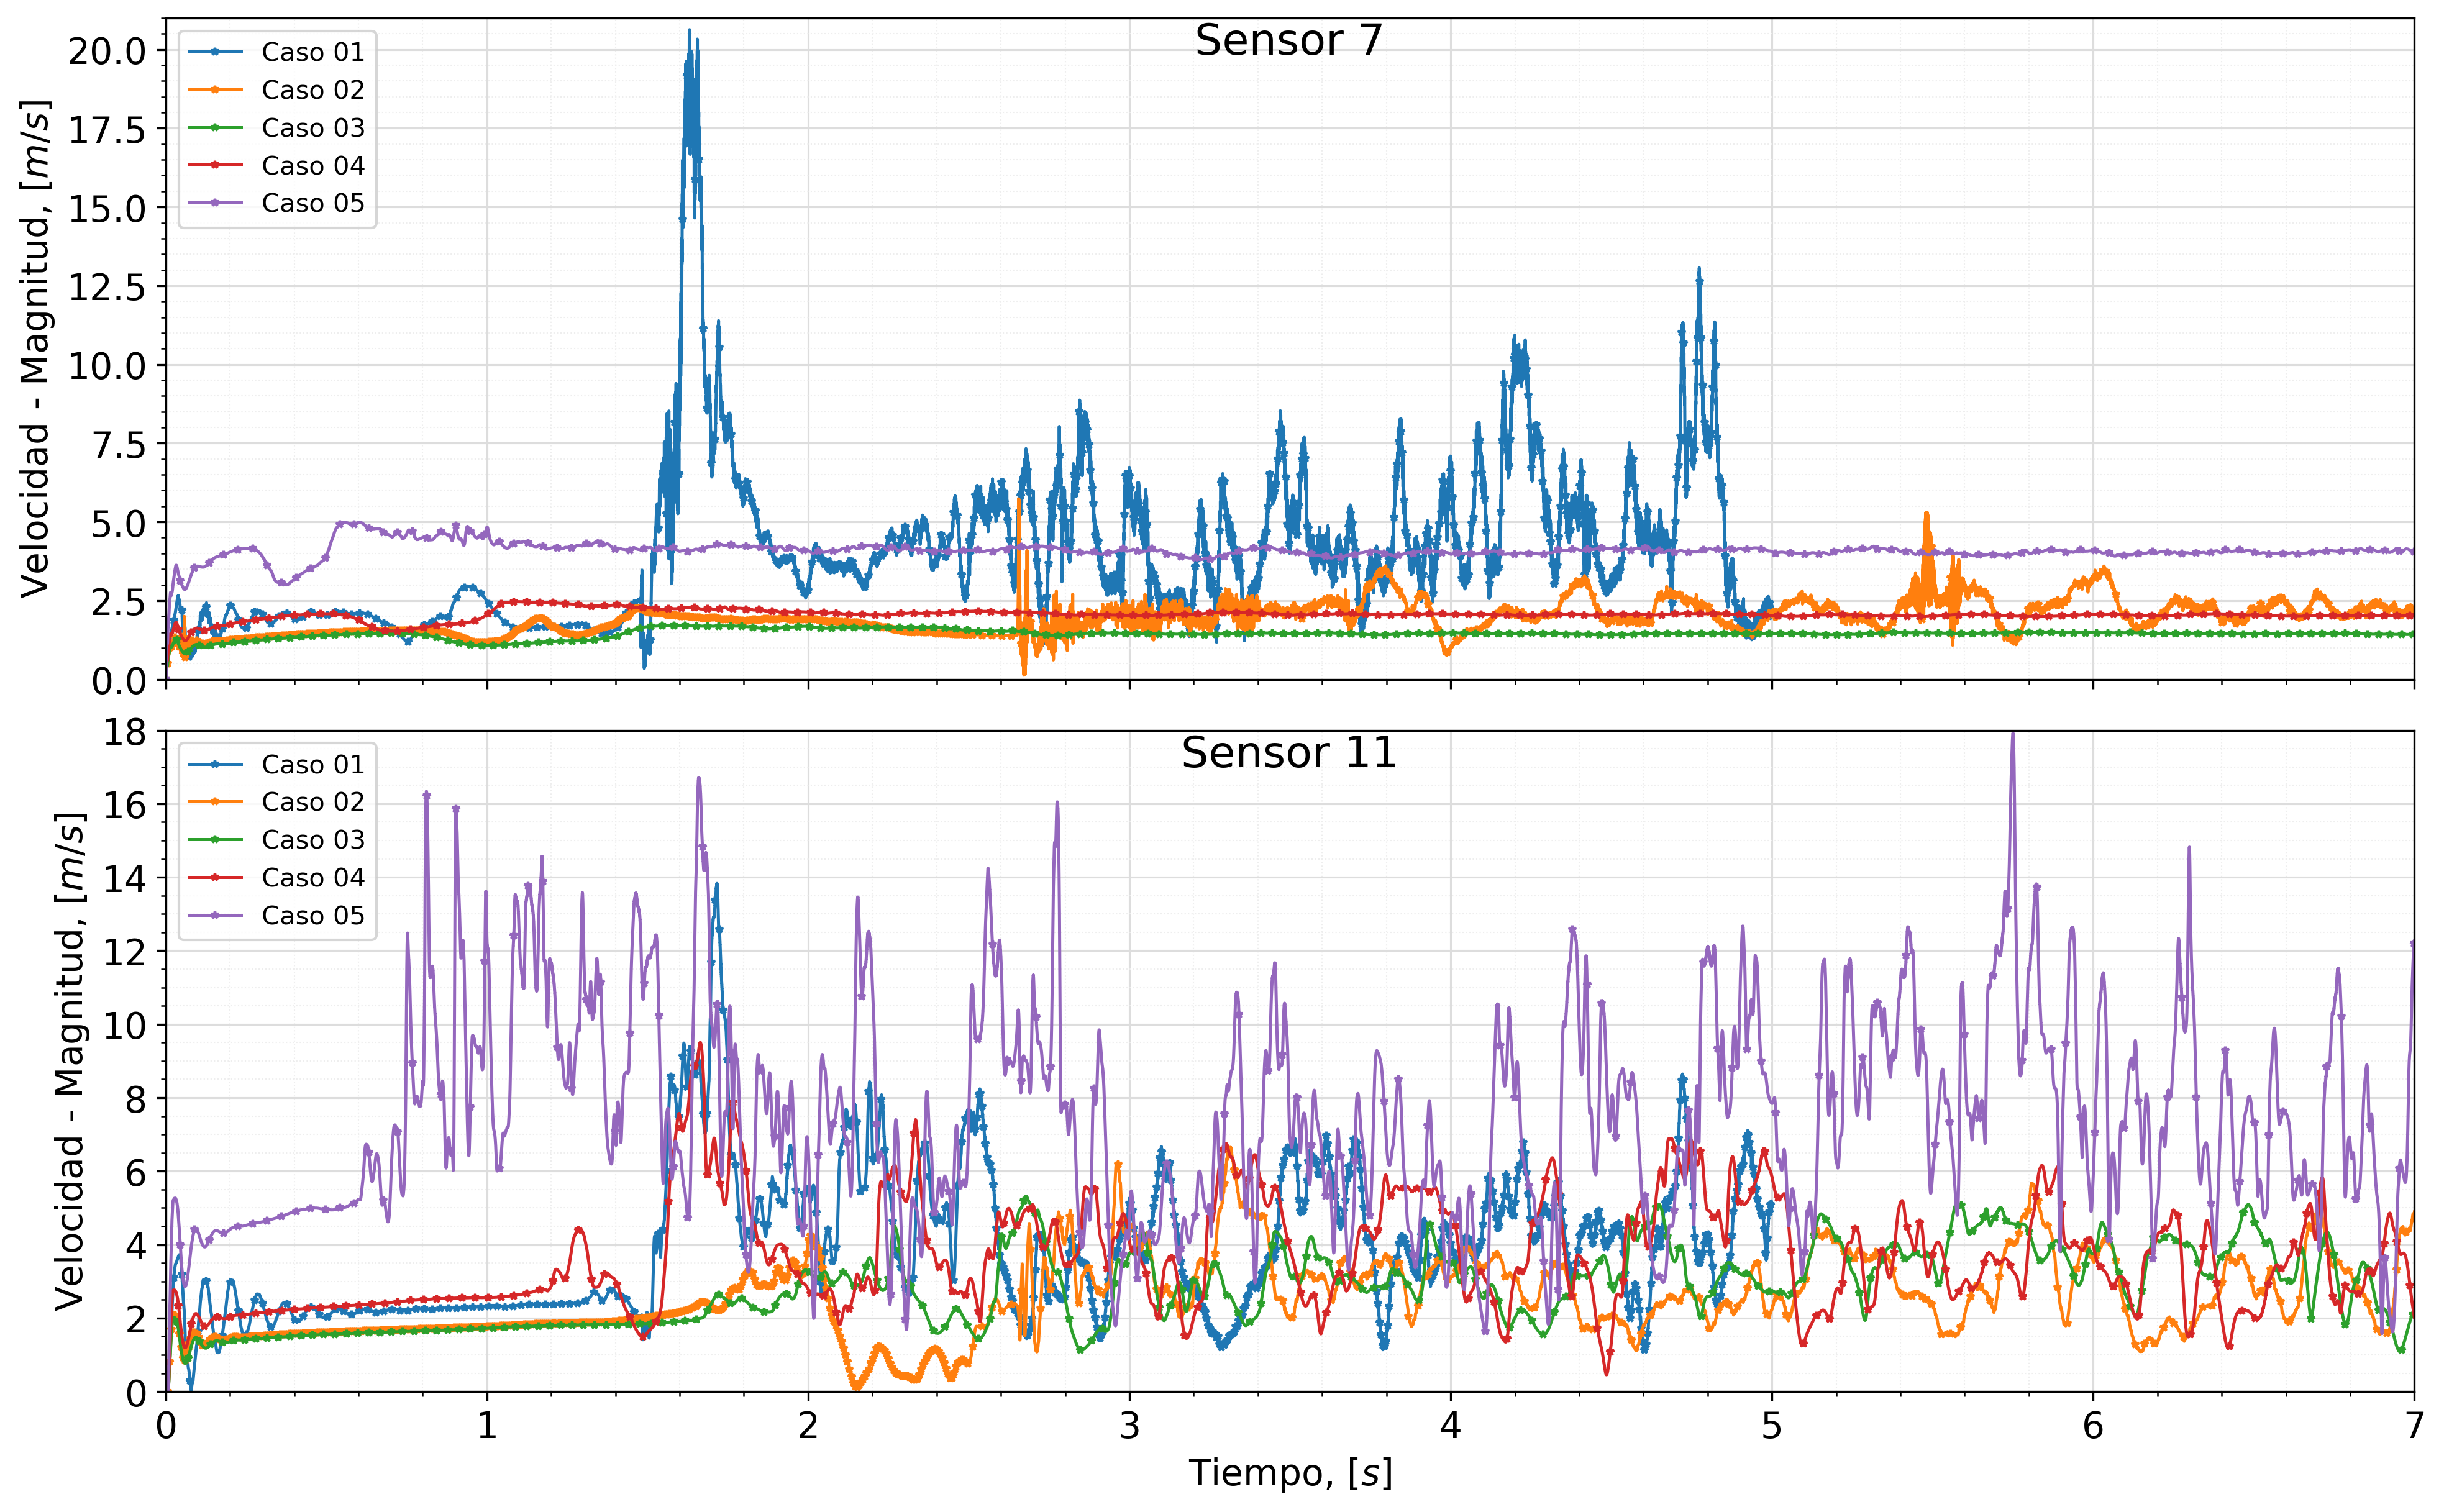
\includegraphics[width=0.75\textwidth]{figures/flowVelocityPlot00.png}
    \end{center}
    \caption{La leyenda de cada figura debe ser un texto corto pero lo
    suficientemente descriptivo de la informaci\'on presentada en la
    figura.}\label{fig:figuraEjemplo00}
\end{figure}

\subsection{Conclusiones}
Cada uno de los casos deber\'a tener una secci\'on de conclusiones donde se
discutan las principales observaciones y hallazgos obtenidos mediante el uso de
modelo matem\'atico-computacional, o del modelo matem\'atico-anal\'itico (si
ese fuese el caso).  Las conclusiones podr\'an incluir apreciaciones acerca de
dificultades en la construcci\'on del modelo, o en la implementaci\'on
computacional que se haya hecho. En cualquier caso, se dar\'a m\'as importancia
a la presentaci\'on de discusiones asociadas al comportamiento del sistema,
fen\'omeno, o proceso explorado en el caso en cuesti\'on. Se evaluar\'a de
manera MUY negativa cualquier tipo de discusi\'on que carezca de
fundamentaci\'on o de apoyo en los resultados presentados en el informe.

\lipsum[1-2]

\section{BIBLIOGRAFÍA}
Cada informe deber\'a incluir una secci\'on de bibliograf\'ia, y el n\'umero de
referencias incluidas y EFECTIVAMENTE utilizadas ser\'a uno de los criterios de
calificaci\'on del informe de taller.

\begin{itemize}

\item \textit{Ferziger, J.H. and Peric, M.}. Computational Methods for Fluid Dynamics.
Springer. Tercera Edición, 2002.
\item \textit{Anderson, J.D.}. Computational Fluid Dynamics: The basics with applications.
McGraw Hill. 1995.
\item \textit{Moukalled, F. et.al.}. The finite volume method in computational fluid
dynamics. Springer. Vol 6. 2016
\item \textit{Hirsch, C.}. Numerical computation of internal \& external flows.
BH-Elsevier. Segunda Edición, 2007.

\end{itemize}

\end{document}          
